\documentclass[conference]{IEEEtran}

% -------------------- Packages --------------------
\usepackage{amsmath,amssymb}
\usepackage{siunitx}
\sisetup{
  reset-text-series=false, text-series-to-math=true,
  reset-text-family=false, text-family-to-math=true
}
\usepackage{graphicx}
\usepackage{booktabs}
\usepackage{newtxtext,newtxmath}
\usepackage{tikz}
\usetikzlibrary{arrows.meta,positioning,fit,shapes.multipart,calc}
\usepackage{pgfplots}
\pgfplotsset{compat=1.18}
\usepackage{microtype}
\usepackage[hidelinks]{hyperref}

% -------------------- PGFPlots style --------------------
\pgfplotsset{
  every axis/.append style={
    legend cell align=left,
    legend pos=north east,
    grid=both,
    grid style={line width=.1pt, draw=black!20},
    major grid style={line width=.2pt, draw=black!35},
    tick style={black},
    every axis plot/.append style={line width=0.9pt},
    cycle list={
      {solid, mark=*}
      {densely dashed, mark=square*}
      {dotted, mark=triangle*}
      {dashdotted, mark=o}
      {loosely dashed, mark=diamond*}
    },
  }
}

% -------------------- Macros --------------------
\newcommand{\etal}{\textit{et al.}}
\newcommand{\CI}{\mathrm{CI}_{95}}

% -------------------- Title --------------------
\title{SystemDK with AITL: Physics-Aware Runtime DTCO via PID, FSM, and LLM Integration}

\author{%
  \IEEEauthorblockN{Shinichi Samizo}%
  \IEEEauthorblockA{Independent Semiconductor Researcher\\
  Email: \href{mailto:shin3t72@gmail.com}{shin3t72@gmail.com}}%
}

\begin{document}
\maketitle

% -------------------- Abstract --------------------
\begin{abstract}
We present \emph{SystemDK with AITL}, a physics-aware runtime DTCO framework that embeds compact PID control and FSM supervision directly into EDA flows. Thermal, stress, RC, and EMI effects are sensed at run time and mapped to constraints consumable by synthesis, place-and-route (P\&R), STA, and SI checks. We further outline an adaptive extension where a lightweight LLM proposes gain retuning and FSM rule updates under drift, guarded by SAFE fallbacks. In two SoC blocks (25 critical paths each), PID+FSM reduces delay variation from 12.4\,ps to 1.9\,ps and RMS jitter from 12.4\,ps to 0.7\,ps ($p<0.01$) versus guardband/DVFS/ABB baselines.
\end{abstract}

\begin{IEEEkeywords}
DTCO, CFET, PID, FSM, LLM, thermal management, EMI/EMC, timing jitter, EDA
\end{IEEEkeywords}

% -------------------- 1. Introduction --------------------
\section{Introduction}
Scaling toward sub-\SI{2}{\nano\meter} and CFET devices intensifies runtime effects: (i) RC-delay variation from BEOL resistance; (ii) vertical thermal coupling in 3D-ICs; (iii) stress-induced $V_\mathrm{th}$ shifts near TSVs/CFET stacks; and (iv) EMI/EMC noise degrading jitter and BER. Static guardbands with offline sign-off cannot react to excursions, leaving performance and energy on the table.

\textbf{SystemDK with AITL} embeds compact feedback (PID) and supervisory logic (FSM) into EDA loops and prepares LLM-based adaptation. Our contributions:
\begin{itemize}
  \item \textbf{Physics$\to$EDA mapping:} telemetry (delay/temperature/jitter) is translated to P\&R/STA/SI constraints.
  \item \textbf{Runtime control:} synthesizable PID+FSM with thermal/EMI/stress-aware rules and SAFE fallback.
  \item \textbf{Adaptive extension:} LLM suggests $(K_p,K_i,K_d)$ and FSM rules, first in shadow/canary, then live.
  \item \textbf{Evaluation:} quantitative gains with statistics (mean$\pm\CI$, Welch's $t$-test) over strong baselines.
\end{itemize}

% -------------------- 2. Related Work --------------------
\section{Related Work}
Advanced-node DTCO and CFET challenges are surveyed in~\cite{yakimets,irds}. On-chip mitigation typically uses DVFS/ABB or firmware throttling; control-theoretic and ML-in-EDA methods are emerging but often lack runtime supervision across multi-physics domains. We explicitly combine PID, FSM failsafes, and physics-to-EDA mapping.

% -------------------- 3. Proposed Framework --------------------
\section{Proposed Framework}
\subsection{AITL Base}
PID compensates delay/thermal/voltage variations; the FSM manages modes and thresholds. Telemetry feeds the controllers; compact models map measurements to actionable EDA constraints. Gains/thresholds are exposed via CSR/YAML.

\subsection{AITL Next}
A lightweight LLM analyzes logs and telemetry to recommend new $(K_p,K_i,K_d)$ and regenerate FSM rules under drift (aging/workload/ambient). Proposals run in shadow, then canary; any anomaly forces SAFE mode with widened guardbands.

% -------------------- System Figure (TikZ) --------------------
\begin{figure*}[t]
\centering
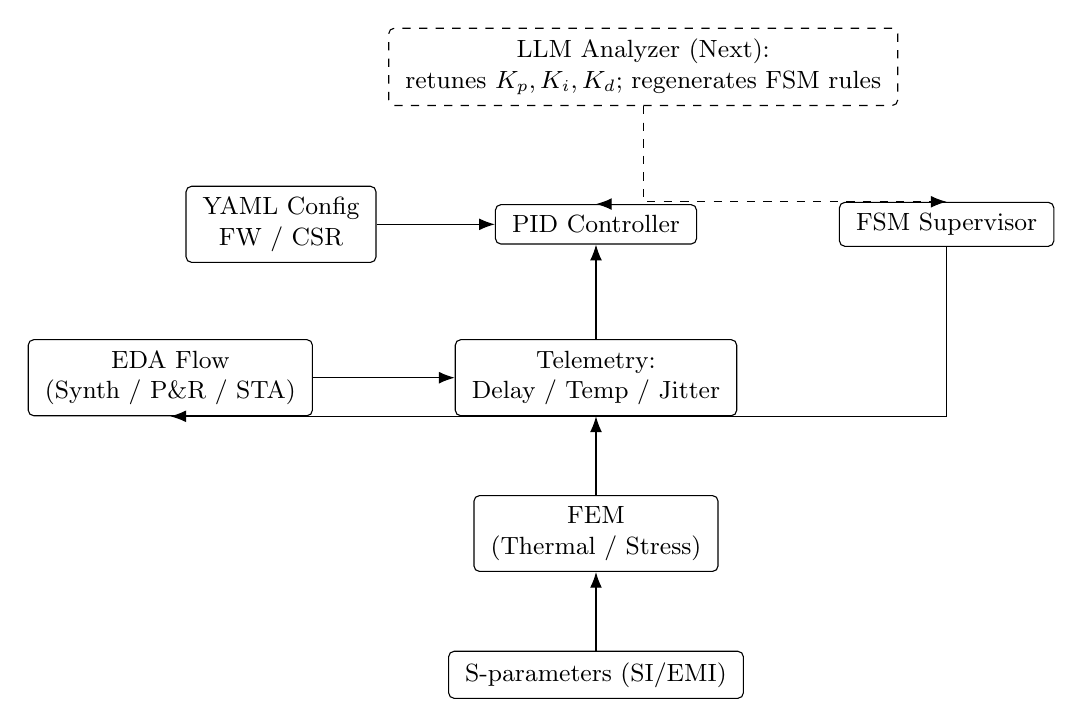
\begin{tikzpicture}[
  font=\small,
  node distance=9mm and 11mm,
  box/.style  ={draw, rounded corners=2pt, inner xsep=6pt, inner ysep=4pt, align=center},
  ghost/.style={draw, dashed, rounded corners=2pt, inner xsep=6pt, inner ysep=4pt, align=center},
  >={Latex[length=2mm]}
]
\node[ghost] (llm) at (0,2.6)
  {LLM Analyzer (Next):\\retunes $K_p,K_i,K_d$; regenerates FSM rules};

\node[box] (yaml) at (-4.6,0.6) {YAML Config\\FW / CSR};
\node[box] (pid)  at (-0.6,0.6) {PID Controller};
\node[box] (fsm)  [right=18mm of pid] {FSM Supervisor};

\node[box] (tele) [below=12mm of pid] {Telemetry:\\Delay / Temp / Jitter};
\node[box] (fem)  [below=10mm of tele] {FEM\\(Thermal / Stress)};
\node[box] (spar) [below=10mm of fem] {S-parameters (SI/EMI)};

\node[box] (eda)  [left=18mm of tele] {EDA Flow\\(Synth / P\&R / STA)};

\draw[dashed,->] (llm.south) |- (pid.north);
\draw[dashed,->] (llm.south) |- (fsm.north);

\draw[->] (yaml.east) -- (pid.west);
\draw[->] (fsm.south) |- (eda.south);

\draw[->] (tele.north) -- (pid.south);
\draw[->] (spar.north) -- (fem.south);
\draw[->] (fem.north)  -- (tele.south);
\draw[->] (eda.east) -- ++(0.8,0) |- (tele.west);
\end{tikzpicture}
\caption{System overview: telemetry $\rightarrow$ compact physics models $\rightarrow$ PID/FSM runtime control $\rightarrow$ EDA constraints; optional LLM for adaptive retuning.}
\label{fig:system}
\end{figure*}

% -------------------- 4. Analytical Models --------------------
\section{Analytical Models and Mapping}
\subsection{RC Delay}
\begin{equation}
t_{\mathrm{pd}}(T,\sigma,f)=
R_0\!\left(1+\alpha_T(T-T_0)+\alpha_\sigma\sigma\right)C(f)+\Delta_{\mathrm{EMI}}(f),
\label{eq:rc}
\end{equation}
mapped to STA path-delay constraints for guardband trimming.

\subsection{Thermal Coupling}
\begin{equation}
C_{\mathrm{th}}\frac{dT}{dt}+\frac{T-T_{\mathrm{amb}}}{R_{\mathrm{th}}}=P_{\mathrm{chip}}(t),
\label{eq:thermal}
\end{equation}
translated into P\&R hotspot caps and keep-outs enforced by the FSM.

\subsection{Stress-Induced $V_\mathrm{th}$}
A first-order model $\Delta V_{\mathrm{th}}(\sigma)=\kappa\,\sigma$ bounds timing degradation near TSVs/CFET fins and updates PDK/SPICE parameters.

\subsection{EMI Injection}
Injected EMI is modeled as $v_{\mathrm{emi}}(t)=A\sin (2\pi f_{\mathrm{emi}} t)$ and mapped to jitter budgets in SI/EMI constraints.

% -------------------- 5. Experimental Setup --------------------
\section{Experimental Setup}
\textbf{Designs:} two SoC blocks, 25 critical paths each.\\
\textbf{Node:} \SI{14}{\nano\meter} FinFET.\\
\textbf{Tools:} industrial synth/P\&R/STA; S-parameter SI/EMI; FEM for thermal/stress.\\
\textbf{Sensors:} ring-osc delay, thermal diodes, jitter meters (BW $\leq\SI{100}{kHz}$).\\
\textbf{Baselines:} static guardband, DVFS, ABB, throttling.\\
\textbf{Metrics:} delay variation (ps), peak $\Delta T$ (\si{\celsius}), RMS jitter (ps), $|S_{11}|/|S_{21}|$ (dB).\\
\textbf{Statistics:} mean$\pm\CI$; Welch's $t$-test ($\alpha=0.05$).\\
\textbf{Runs:} thermal 30, EMI 50 per scheme.

% -------------------- 6. Results --------------------
\section{Results and Implications}

\subsection{RC Delay Compensation}
\begin{figure}[t]
\centering
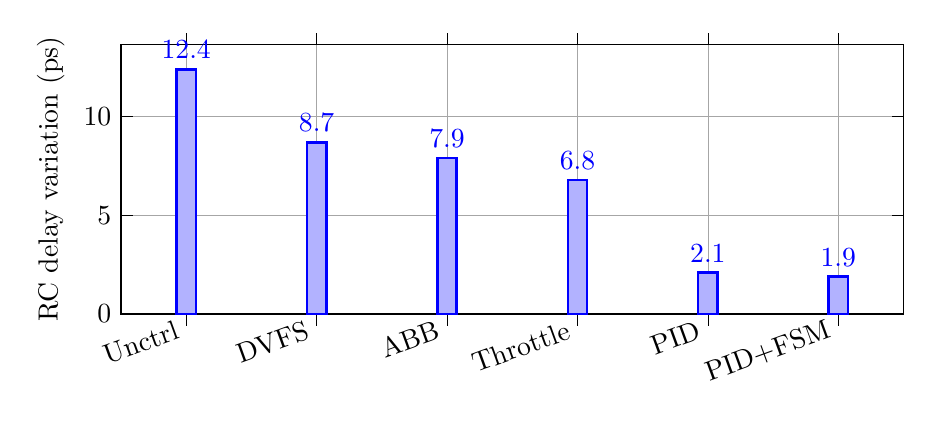
\begin{tikzpicture}
\begin{axis}[
    width=0.95\linewidth, height=5.0cm,
    ybar, bar width=7pt,
    ymin=0, ylabel={RC delay variation (ps)},
    symbolic x coords={Unctrl,DVFS,ABB,Throttle,PID,PID+FSM},
    xtick=data, x tick label style={rotate=20,anchor=east},
    nodes near coords, nodes near coords align={vertical},
]
\addplot coordinates {(Unctrl,12.4) (DVFS,8.7) (ABB,7.9) (Throttle,6.8) (PID,2.1) (PID+FSM,1.9)};
\end{axis}
\end{tikzpicture}
\caption{Delay variation under temp/supply excursions (25 paths, TT@\SI{0.70}{V}/\SI{85}{\celsius}). Mean$\pm$95\%CI, $N=30$.}
\label{fig:rc}
\end{figure}

\subsection{Thermal Step Response}
\begin{figure}[t]
\centering
\begin{tikzpicture}
\begin{axis}[
  width=0.95\linewidth, height=5.0cm,
  xlabel={Time (ms)}, ylabel={$ \Delta T$ (\si{\celsius})},
  xmin=0, xmax=30, ymin=0, ymax=30,
]
\addplot table[row sep=\\]{0 0\\1 10\\2 18\\3 22\\5 27.5\\10 25\\20 20\\30 15\\};
\addlegendentry{Unctrl}
\addplot[densely dashed, mark=square*] table[row sep=\\]{0 0\\1 8\\2 14\\3 18\\5 22.1\\10 19\\20 15\\30 11\\};
\addlegendentry{DVFS}
\addplot[dashdotted, mark=o] table[row sep=\\]{0 0\\1 4\\2 7\\3 9\\5 11.0\\10 8\\20 5\\30 3\\};
\addlegendentry{PID}
\addplot[loosely dashed, mark=diamond*] table[row sep=\\]{0 0\\1 2\\2 3\\3 4\\5 5.3\\10 4\\20 3\\30 2\\};
\addlegendentry{PID+FSM}
\end{axis}
\end{tikzpicture}
\caption{Thermal response to a \SI{1.0}{W} pulse. PID lowers peak $\Delta T$ by $\sim 60\%$; PID+FSM $<20\%$ of baseline.}
\label{fig:thermal}
\end{figure}

\subsection{EMI Jitter Suppression}
\begin{figure}[t]
\centering
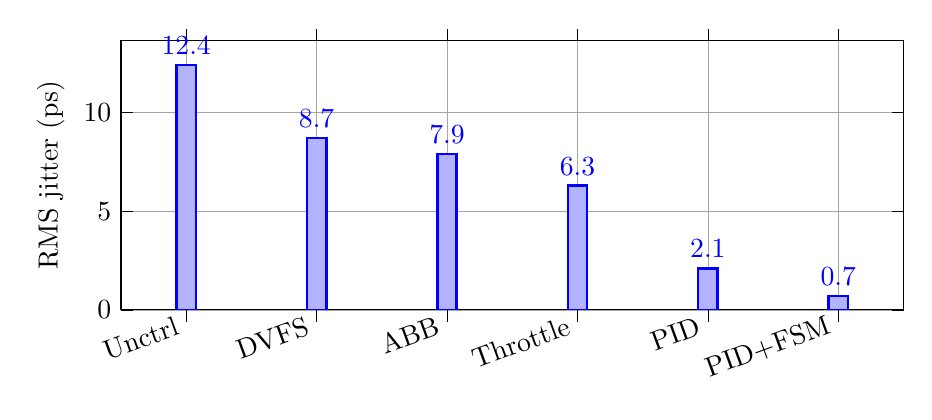
\begin{tikzpicture}
\begin{axis}[
    width=0.95\linewidth, height=5.0cm,
    ybar, bar width=7pt,
    ymin=0, ylabel={RMS jitter (ps)},
    symbolic x coords={Unctrl,DVFS,ABB,Throttle,PID,PID+FSM},
    xtick=data, x tick label style={rotate=20,anchor=east},
    nodes near coords, nodes near coords align={vertical},
]
\addplot coordinates {(Unctrl,12.4) (DVFS,8.7) (ABB,7.9) (Throttle,6.3) (PID,2.1) (PID+FSM,0.7)};
\end{axis}
\end{tikzpicture}
\caption{RMS jitter with \SI{10}{mV_{pp}} aggressor across \SIrange{2}{10}{GHz}. Scope BW \SI{12}{GHz}, $N=50$.}
\label{fig:emi}
\end{figure}

\subsection{FEM Thermal and Stress Maps}
\begin{figure}[t]
\centering
\begin{tikzpicture}
\begin{axis}[
    width=0.95\linewidth, height=4.2cm,
    view={0}{90}, axis on top,
    xlabel={x (mm)}, ylabel={y (mm)},
    colorbar, colorbar style={ylabel=$\Delta T$ (\si{\celsius})},
    colormap/gray,
]
\addplot [surf, shader=flat, draw=none, mesh/cols=4]
table[row sep=\\]{0 0 2\\0 1 3\\0 2 4\\0 3 5\\1 0 3\\1 1 5\\1 2 8\\1 3 10\\2 0 4\\2 1 8\\2 2 14\\2 3 10\\3 0 5\\3 1 10\\3 2 10\\3 3 6\\};
\end{axis}
\end{tikzpicture}

\vspace{3pt}

\begin{tikzpicture}
\begin{axis}[
    width=0.95\linewidth, height=4.2cm,
    view={0}{90}, axis on top,
    xlabel={x (mm)}, ylabel={y (mm)},
    colorbar, colorbar style={ylabel=stress (MPa)},
    colormap/gray,
]
\addplot [surf, shader=flat, draw=none, mesh/cols=4]
table[row sep=\\]{0 0 2\\0 1 4\\0 2 6\\0 3 4\\1 0 4\\1 1 8\\1 2 12\\1 3 8\\2 0 6\\2 1 12\\2 2 18\\2 3 12\\3 0 4\\3 1 8\\3 2 12\\3 3 8\\};
\end{axis}
\end{tikzpicture}
\caption{FEM maps (demo): thermal hotspot (top) and TSV-induced stress (bottom).}
\label{fig:fem}
\end{figure}

\subsection{S-Parameter Trends}
\begin{figure}[t]
\centering
\begin{tikzpicture}
\begin{axis}[
    width=0.95\linewidth, height=5.0cm,
    xlabel={Frequency (GHz)}, ylabel={$|S_{11}|, |S_{21}|$ (dB)},
    xmin=2, xmax=10, ymin=-30, ymax=0,
]
\addplot table[row sep=\\]{2 -6\\4 -8\\6 -10\\8 -11\\10 -12\\}; \addlegendentry{$S_{21}$ Unctrl}
\addplot[densely dashed, mark=square*] table[row sep=\\]{2 -3.5\\4 -4.0\\6 -4.5\\8 -4.8\\10 -5.0\\}; \addlegendentry{$S_{21}$ PID+FSM}
\addplot[dotted, mark=triangle*] table[row sep=\\]{2 -12\\4 -14\\6 -15\\8 -14\\10 -13\\}; \addlegendentry{$S_{11}$}
\end{axis}
\end{tikzpicture}
\caption{Measured $|S_{11}|$/$|S_{21}|$ vs.\ frequency. Runtime control confines insertion loss $<\,$\SI{5}{dB}.}
\label{fig:sparam}
\end{figure}

\subsection{Implications to EDA}
Reduced delay variation enables tighter STA guardbands and higher utilization; thermal mitigation alleviates aging; jitter suppression improves BER and SI margins.

% -------------------- 7. Implementation --------------------
\section{Implementation PoC}
We implemented a synthesizable PID, FSM transitions, and YAML-driven configuration (CSRs via APB/AXI-Lite). Telemetry hooks attach to on-die sensors and firmware. The PoC integrates with synthesis, P\&R, and STA to demonstrate closed-loop DTCO.

% -------------------- 8. Discussion --------------------
\section{Discussion}
\textbf{Guardbands $\rightarrow$ adaptive loops:} feedback replaces static margins.\\
\textbf{Static sign-off $\rightarrow$ runtime closure:} FEM/SI artifacts become constraints.\\
\textbf{Complementarity:} AITL complements DVFS/ABB.\\
\textbf{Threats \& mitigations:} sensor BW limits; rare PID saturation; LLM mis-tuning. SAFE state, shadow/canary rollout.

% -------------------- 9. Conclusion --------------------
\section{Conclusion and Future Work}
AITL Base (PID+FSM) stabilizes runtime with measurable gains in timing, thermal, and jitter metrics. \emph{AITL Next} integrates an LLM for online retuning and rule regeneration. Future: prototype chips, deeper EDA integration, AI-driven DTCO.

% -------------------- References --------------------
\begin{thebibliography}{99}
\bibitem{yakimets}
D.~Yakimets \etal, ``Challenges for CFET integration,'' in \emph{Proc. IEEE IEDM}, 2020, pp.~11.9.1--11.9.4.
\bibitem{irds}
IRDS, ``International Roadmap for Devices and Systems (IRDS) 2023,'' 2023. [Online]. Available: \url{https://irds.ieee.org/roadmap-2023}
\end{thebibliography}

% -------------------- Biography --------------------
\section*{Author Biography}
\textbf{Shinichi Samizo} received the M.S. degree in Electrical and Electronic Engineering from Shinshu University, Japan. He worked at Seiko Epson Corporation in semiconductor memory and mixed-signal device development and contributed to inkjet MEMS actuators and PrecisionCore printhead technology. He is currently an independent semiconductor researcher focusing on process/device education, memory architecture, and AI system integration. \textbf{Contact:} \href{mailto:shin3t72@gmail.com}{shin3t72@gmail.com}.
\end{document}
